\subsection{Deep Q-learning} \label{basics}

In this second section of the first part, we present deep Q-learning, a variant of the aforementioned method combining the Q-learning algorithm with deep learning. Here, deep Q-learning, or DQN, does not refer to one algorithm, but a family of algorithms, among which the seven main ones are known as rainbow DQN [3] (Hessel et al., 2017). Four of those have been implemented as part of this internship, and are discussed here.

\subsubsection{DQN: Vanilla Deep Q-learning} \label{basics}

\textbf{From discrete to continuous state spaces} \\
For a long time, Q-learning has been restricted to its tabular version, and thus, to toy problems. In fact, the discretization of the state space and its storage in a table causes a major problem, i.e. the absence of generalization between states. In the Q-table, each Q-value is estimated separately, and must be updated many times for optimization. As the states represent combinations of multi-dimensional features, the MDP and the Q-table grow exponentially large with the state space, as every state encountered is virtually a new state. Thus, discrete representations of continuous problems are mostly impossible, the cost of exploring fine discrete states is immensely high, while the lack of details impedes learning when exploiting coarse discrete states. Several propositions have been considered for using Q-learning with continuous function approximators, such as genetic algorithms, support vector machines and shallow networks, however without significant improvements. In particular, neural networks seemed an appealing solution for approximating the Q-function, but it was found that non-linear approximators make Q-learning unstable and diverge in practice. Neural network based Q-learning was thought to be an insoluble problem for decades, until the rise of deep learning in the recent years allowed researchers at Google DeepMind to came up in 2015 with the deep Q-network, or DQN. \\

\textbf{Neural networks are continuous function approximators} \\
A neural network is a collection of interconnected artificial neurons, called perceptrons, approximating a function by mapping input data vectors to outputs. The simplest architecture for neural networks is the multi-layered perceptron (MLP), or simply artificial neural network (ANN), and is composed of $L$ successive layers of $s_l$ perceptrons. Each neuron from a layer $l$ is connected to all the neurons in the next layer $l+1$, and propagates an activation signal in the activation signal matrix $a$ through the network. The node $(l+1,i)$, the perceptron $i$ at layer $l+1$, acts like a simple mathematical unit and performs two operations, a dot product between the activation signals $a^{(l)}$ emitted by the previous layer and a set of weights $\Theta^{(l)}$ controlling the function mapping within the cross-layer connections and an additional bias unit, and a non-linear activation function $g^{(l)}$ on the resulting scalar $z$, then propagates the activation signal $a^{(l+1)}_i$ to the next layer: 
\[ a^{(l+1)}_i = g^{(l)}(z) \text{, with } z = \sum_{j=0}^{s_{l}} \Theta^{(l)}_{i,j} \cdot a^{(l)}_{j} \]
The input layer receives the raw input as activation, so that $a^{(1)} = X$. The activation function depends on the task and the depth in the network. In hidden layers, $g(l)$ is often the ReLU activation, or one of its variants, a rectifier linear unit, while the output layer can have $g(L-1)$ a sigmoid or tanh activation for binary classification (logistic regression), a softmax activation for multi-class classification, or no activation for raw output:
\[ ReLU(z) = \max(0,z) \text{, } sigmoid(z) = \frac{1}{1+e^{-z}}  \text{, } softmax(z)_i = \frac{e^{z_i}}{\sum_{j=1}^K e^{z_j}} \]
The whole propagation of a signal from the input layer through the output layer is the forward propagation, its result is a hypothesis $h_{\Theta}^{(m)} = a^{(L)}$ over the input training data $m$, and is performed over multiple inputs from a batch of $M$ training data. The neural network is a supervised learning tool, and uses labeled data to learn from the hypotheses. A loss function $L(y,h_{\Theta})$ measures the error between the batch of hypotheses $h_{\Theta}$ computed by forward propagation and the batch of corresponding real values $y$ of the outputs. The most common loss function is the L2-loss, the mean square error loss function (MSE):
\[ L(y,h_{\Theta}) = \frac{1}{2M}\sum_{m=1}^M (y^{(m)} - h_{\Theta}^{(m)})^2 \]
The goal of training a neural network is to minimize the loss function with respect to the weights, i.e. correcting the weights $\Theta_{i,j}^{(l)}$ in the network so that $L(y,h_{\Theta}) \rightarrow \min_{\Theta} L(y,h_{\Theta})$. An error term $\Delta_{i,j}^{(l)}$ is computed for all the weights by deriving the gradient of the loss function and the additional L2-norm $R(\Theta, \lambda)$ regularization term, over the weights $\Theta_{i,j}^{(l)}$:

\[ \Delta_{i,j}^{(l)} = \frac{\partial}{\partial \Theta_{i,j}^{(l)}} (L(y,h_{\Theta}) + R(\Theta, \lambda)) \text{, with } R(\Theta, \lambda) = \frac{\lambda}{2M}\sum_{l=1}^{L-1}\sum_{i=1}^{s_l}\sum_{j=1}^{s_{l+1}}(\Theta_{i,j}^{(l)})^2 \]

In practice, the gradient is computed by numerical approximations for each neuron, by propagating the error terms from the output layer to the input layer, the back propagation. It is during the back propagation that the weights $\Theta_{i,j}^{(l)}$ are corrected with an optimizer by the error $\Delta_{i,j}^{(l)}$ and a learning rate $\alpha$. This optimizer is the gradient descent algorithm:
\[ \Theta_{i,j}^{(l)} = \Theta_{i,j}^{(l)} - \alpha \cdot \Delta_{i,j}^{(l)} \]

Learning in a neural networks thus consists of approximating a function by mapping from input training data to output labels, through many forward and backward passes in layers of interconnected neurons, by measuring the average loss over batches of hypotheses and target values, and correcting the errors in the connection's weights with gradient descent. \\

\begin{SCfigure}[0][h]
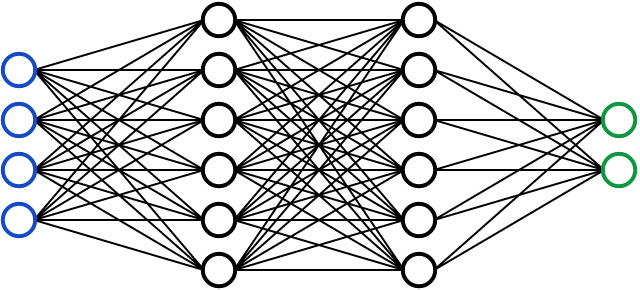
\includegraphics[scale=0.5]{img/I/Selection_098.png}
\centering
\caption{MLP.}
\end{SCfigure}

\textbf{Neural networks are unstable in Q-learning} \\
In Q-learning, neural networks are met with two primary issues that are inherent to RL. \\
(1) Successively correlated data; in supervised learning, data are inferred randomly from a prepared data set, and, while coming from the same data distribution, successive samples are not directly correlated. In Q-learning however, the data come from the observations of state transitions $(s,a,s',r')$ in a time sequence, and are thus highly successively correlated. This causes catastrophic forgetting, a phenomenon where the neural network over-fits to new experiences and unlearns old training, after having significantly changed the weights.
(2) Moving targets; in supervised learning, target values are labeled beforehand, and are therefore the exact and definitive values of optimal hypotheses. In Q-learning however, the targets are constructed dynamically by temporal difference from the Q-values. These estimates vary depending on the Q-function, that is iteratively updated through learning. While only the specific Q-value $Q_{\pi}(s,a)$ is updated at the given transition with a Q-table, a neural network updates all its weights at each back propagation pass, thus updating all the Q-values $Q_{\pi}(s,a)$ of the Q-function. Consequently, the estimated temporal difference targets are constantly changing, or moving, and any update can deeply alter the policy.
Because of (1) and (2), NN-based Q-learning has been known to be unstable and diverge. \\

\textbf{Deep Q-network, replay memory and target network} \\
In [4,5] (Mnih et al., 2015), the authors propose the deep Q-network algorithm (DQN), a convergent solution to Q-learning with a neural network as the Q-function approximator, later referred to as the vanilla DQN algorithm, i.e. as part of the rainbow DQN family. \\
Here, the Q-network $Q$ with weights $\Theta$ is a Q-function approximator such that $Q_{\pi}(s,a,\Theta) \approx Q^*_{\pi}(s,a)$, a neural network mapping from one state $s$ to all the Q-values $Q_{\pi}(s,a,\Theta), \forall a \in A$ for this state. The input layer is an $|s|$-dimensional vector, for the $|s|$ features of state $s$ in the continuous action space $S$, and the ouput layer is an $|A|$-dimensional vector, for the $|A|$ Q-values $Q_{\pi}(s,a,\Theta)$ of the $|A|$ possible actions $a$ in the discrete action space $A$, with $a = arg\max_a Q_{\pi}(s,a,\Theta)$ the optimal action to take following the optimal policy $\pi^*(s,a)$. \\
The two aforementioned problems causing the instability of neural networks as Q-function approximators are tackled with two novel key ideas, one respectively for each problem.
On the one hand, the replay memory addresses (1) the successively correlated data issue. The replay memory $D$ is a data buffer storing the $N$ last transitions experienced by the agent, $D = \{e_{t-1},e_{t-2},...,e_{t-N}\} \text{, with } e_t = (s_t,a_t,s_{t+1},r_{t+1})$. At each time step $t$, the agent stores the experienced transition $e_t$ in the replay memory, without updating the Q-network. It then draws uniformly at random $M$ past transitions from the replay memory, and performs an update of the Q-network by back propagation over this batch $U(D)$. Before the beginning of learning, the replay memory is filled with random transitions, i.e. transitions with only random actions taken, following an $\epsilon$-greedy policy with $\epsilon=1$. Hence, the bigger $N$ the size of the replay memory, the lower the correlation probability. \\
On the other hand, the target network addresses (2) the moving targets issue. The target $\hat{Q}$-network $\hat{Q}$ with weights $\Theta^-$ is a second neural network, copied from the online $Q$-network periodically every $C$ steps, such that $\Theta^-_t = \Theta_{\lfloor \frac{t}{C} \rfloor \cdot C}$, with $C$ the update target frequency. The target $\hat{Q}$-network is never updated by gradient optimization, and its weights $\Theta^-$ are held fixed and used for generating fixed temporal difference targets $y_t$ for the $C$ next updates of the online $Q$-network, introducing a delay that reduces divergence. \\
With the online $Q$-network $Q$, the replay memory $D$ and the target $\hat{Q}$-network $\hat{Q}$, DQN provides a stable model for approximating continuous Q-functions with neural networks. \\

\textbf{Vanilla DQN algorithm} \\
In the vanilla DQN algorithm, the $Q$-network replaces the Q-table as the Q-function approximator. The algorithm is as follows: The online $Q$-network $Q$ is initialized with random weights $\Theta_0$, and the target $\hat{Q}$-network $\hat{Q}$ is initialized with copied weights $\Theta^-_0=\Theta_0$. The replay memory buffer $D$ is initialized with capacity $N$, and  filled with $N_{min} \leq N$ random transitions, with random actions taken. For $E$ episodes, over the sequences from an initial to a terminal state, with total steps $t$, the agent observes the state $s_t=\phi(x_t)$, from observation $x_t$ and pre-processing function $\phi$, takes the action $a_t$ by Q-values $Q_{\pi,t}(s_t,a,\Theta_t)$ from forward propagation through the online $Q$-network $Q$ and according to the $\epsilon$-greedy policy, and the model transitions to the next state $s_{t+1}$, yielding reward $r_{t+1}$. The transition $(s_t,a_t,s_{t+1},r_{t+1})$ is stored in the replay memory buffer $D$, and a sample batch $U(D)$ of $M$ past transitions is drawn uniformly at random from the pool of stored experiences. The target $y^{(m)}_t$, the temporal difference target by forward propagation through the target $\hat{Q}$-network $\hat{Q}$, and the hypothesis $h_{\Theta,t}^{(m)}$, the Q-value by forward propagation through the online $Q$-network $Q$, are computed for each transition $(s,a,s',r')^{(m)}$ in the batch $U(D)$:
\[ y^{(m)}_t = r'^{(m)} + \gamma \cdot \max_{a'}Q_{\pi,t}(s'^{(m)},a',\Theta^-_t) \text{, } h_{\Theta,t}^{(m)} = Q_{\pi,t}(s^{(m)},a^{(m)},\Theta_t) \]
The online $Q$-network $Q$ is updated by back propagation with a gradient descent step on the gradient $\Delta_t$ derived from the MSE loss over the temporal differences $\delta^{(m)}_t = y^{(m)}_t - h_{\Theta,t}^{(m)}$:
\[
\begin{split}
 L_t(y_t,h_{\Theta,t}) &= \frac{1}{2M}\sum_{m=1}^M (y^{(m)}_t - h_{\Theta,t}^{(m)})^2 = L_t(\delta_t) = \frac{1}{2M}\sum_{m=1}^M (\delta_t^{(m)})^2 \\
 &= \frac{1}{2M}\sum_{m=1}^M (r'^{(m)} + \gamma \cdot \max_{a'}Q_{\pi,t}(s'^{(m)},a',\Theta^-_t) - Q_{\pi,t}(s^{(m)},a^{(m)},\Theta_t))^2
\end{split}
\]
Finally, the weights $\Theta^-$ of the target $\hat{Q}$-network $\hat{Q}$ are reset by copy of the weights $\Theta$ of the online $Q$-network $Q$ every $C$ steps, such that $\Theta^-_t = \Theta_t$ and $\hat{Q}_t = Q_t$ if $t \equiv 0 \pmod{C}$.

\begin{algorithm}[H]
\small
\caption*{Vanilla DQN algorithm}
\begin{algorithmic}
    \STATE Initialize step $t = 0$;
    \STATE Initialize the online $Q$-network $Q$ with random weights $\Theta_0$;
    \STATE Initialize the target $\hat{Q}$-network $\hat{Q}$ with weights $\Theta^-_0 = \Theta_0$;
    \STATE Initialize the replay memory buffer $D$ to capacity $N$
    \STATE with $Nmin$ random transitions $(s,\text{rand }a \in A,s',r')$;
    \FOR{episode e = 1:E}
        \bindent
        \STATE Initialize sequence, observe initial state $s_t=\phi(x_t)$;
        \WHILE{$s_t$ not terminal}
            \bindent
            \STATE With probability $\epsilon$ select a random action $a_t \in A$
            \STATE otherwise select action $a_t = arg\max_{a}Q_{\pi,t}(s_t,a,\Theta_t)$;
            \STATE Execute $a_t$ in emulator $\varepsilon$ and observe reward $r_{t+1}$ and next state $s_{t+1}=\phi(x_{t+1})$;
            \STATE Store transition $(s_t,a_t,s_{t+1},r_{t+1})$ in $D$;
            \STATE Sample random batch $U(D)$ of $M$ transitions $(s,a,s',r')^{(m)}$ in $D$;
            \FOR{m = 1:M}
                \bindent
                \STATE Set TD error $\delta^{(m)}_t = r'^{(m)} + \gamma \cdot \max_{a'}Q_{\pi,t}(s'^{(m)},a',\Theta^-_t) - Q_{\pi,t}(s^{(m)},a^{(m)},\Theta_t)$;
                \eindent
            \ENDFOR
            \STATE Perform a gradient descent step on MSE loss $L_t(\delta_t)$ w.r.t. $\Theta_t$,  with $\Delta_t$, $\alpha$;
            \IF{$t \equiv 0 \pmod{C}$}
                \bindent
                \STATE Reset target $\hat{Q}$-network $\hat{Q} = $ online $Q$-network $Q$, with $\Theta^-_t = \Theta_t$;
                \eindent
                \ENDIF
            \STATE Decay $\epsilon$ with linear decay;
            \STATE Increment step $t = t + 1$;
            \eindent
        \ENDWHILE
        \eindent
    \ENDFOR
\end{algorithmic}
\end{algorithm}

\textbf{Deep Q-learning converges, but is not optimized} \\
At this point, vanilla DQN provides a convergent model to approximate continuous Q-functions with neural networks in Q-learning. It is however not optimized, and extremely sample inefficient, requiring millions of time frames to optimize a Q-function, sometimes tens or hundreds of millions. The optimization of deep Q-learning algorithms has therefore become an active field of research in recent years, with many proposed improvements. \\
The rainbow DQN family lists six extensions that significantly improve specific aspects of the original vanilla DQN algorithm, towards a stabler and faster learning. Furthermore, these enhancements have been chosen to be mutually inclusive, and can be combined for better results, with each combination being virtually a new and functional DQN variant. \\
Three of these upgrades have been studied during this internship, and implemented together on top of the vanilla DQN to arrive at the algorithm used for the internship project.

\subsubsection{DDQN: Double Deep Q-learning} \label{basics}

\textbf{Overestimation in the TD target values} \\
DQN uses the temporal difference to build the target values $y_t$ from the target $\hat{Q}$-network $\hat{Q}$ in the loss function. However, in $max_{a'}Q_{\pi,t}(s',a',\Theta^-_t)$, the same $max$ operator both selects the action and evaluates the estimated Q-value for the temporal difference target. This maximization step is prone to favoring overestimated Q-values over underestimated ones, and results in overoptimistic Q-value estimates. DQN thus tends to develop unrealistically high value functions in the Q-function, thereby learning sub-optimal policies. \\

\textbf{Decoupling action selection and action evaluation} \\
In [6] (Hasselt et al., 2015), the authors present the double deep Q-network (DDQN) algorithm, effectively reducing overestimation by decoupling the selection of the action and the evaluation of the Q-value in the temporal difference target. In a two-step process, hence "double", the estimated optimal action is first selected by forward propagation through the online $Q$-network $Q$, and the corresponding estimated Q-value is then evaluated by forward propagation through the target $\hat{Q}$-network $\hat{Q}$. The TD target is thus re-written:
\[ y_t = r' + \gamma \cdot Q_{\pi,t}(s',arg\max_{a'}Q_{\pi,t}(s',a',\Theta_t),\Theta^-_t) \]

\subsubsection{3DQN: Dueling Double Deep Q-learning} \label{basics}

\textbf{Exploration efficiency and irrelevant actions} \\
In continuous state spaces, for many states, some actions do not affect the environment in any relevant way, and it is unnecessary to estimate the value of each action choice. In Q-learning however, the action-value function is an estimate of the value function over a specific action, and do not differentiate the value of being in a state and the advantage of taking an action from this state. The Q-network must thus estimate the state values for every state to choose an optimal action, assessing the inherent values of actions in respect to the Q-values only in retrospect. This causes DQN to be extremely sample inefficient, requiring long exploration times to derive good policies, i.e. tens of millions of samples. \\

\textbf{Decoupling value and advantage with the advantage function} \\
The dueling double DQN (3DQN) algorithm [7] (Wang et al., 2016), with its dueling network architecture, can learn which states are, and are not, valuable, without having to learn each action for each state, by decoupling the state values and the action advantages into value function $V_\pi(s)$ and advantage function $A_\pi(s,a)$. The dueling architecture learns a general state value that is shared across similar actions, leading to faster convergence and more efficient Q-functions. The Q-function measures the value of taking action $a$ being in state $s$, the V-function measures the value of being in state $s$, and the A-function measures the relative advantage of taking action $a$ deducing the value of being in state $s$:
\[ 
\begin{cases}
  Q_\pi(s,a) = V_\pi(s) + A_\pi(s,a) \\
  V_\pi(s) = \mathbf{E}_{\pi}[Q_\pi(s,a)|\pi] & \implies A_\pi(s,a) = Q_\pi(s,a) - V_\pi(s)\\
  \mathbf{E}_{\pi}[A_\pi(s,a)|\pi] = 0
\end{cases}
\]

\textbf{Dueling Q-network architecture} \\
The 3DQN algorithm introduces a novel neural network architecture specifically designed for value-based reinforcement learning, the dueling Q-network. A final hidden layer is added after the main network learning module, with weights $\Theta_t$, splitting the propagated signal into two streams for the value function and the advantage function. The $1$-dimensional value stream, with weights $\kappa_t$, estimates the scalar state value $V_{\pi,t}(s,\Theta_t,\kappa_t)$, and the $|A|$-dimensional advantage stream, with weights $\iota_t$, estimates the action advantage value vector $A_{\pi,t}(s,a,\Theta_t,\iota_t)$,  $\forall a \in A$. The value and advantage streams are combined to produce the Q-function $Q_{\pi,t}(s,a,\Theta_t,\iota_t,\kappa_t)$ in a special aggregation output layer, with:
\[ Q_{\pi,t}(s,a,\Theta_t,\iota_t,\kappa_t) = V_{\pi,t}(s,\Theta_t,\kappa_t) + (A_{\pi,t}(s,a,\Theta_t,\iota_t) - \frac{1}{|A|}\sum_{a'}A_{\pi,t}(s,a',\Theta_t,\iota_t)) \]

\begin{SCfigure}[0.1][h]
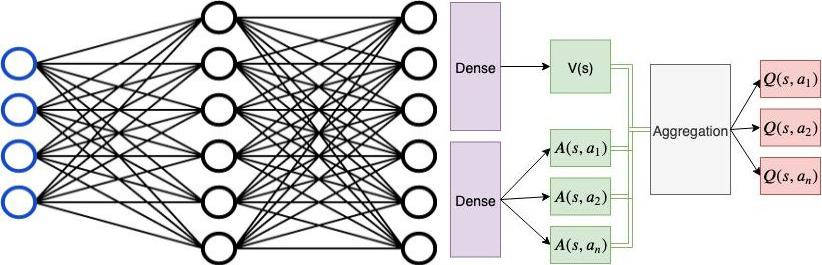
\includegraphics[scale=0.63]{img/I/Dueling-Q-architecture.jpg}
\centering
\caption{Dueling DQN.}
\end{SCfigure}

\subsubsection{Per3DQN: 3DQN with Prioritized Experience Replay} \label{basics}

\textbf{Exploitation efficiency and random transition sampling} \\
DQN uses an an experience replay memory buffer to store a pool of past experiences in the form of $(s,a,s',r')$ transitions, to solve the successively correlated data issue occurring when transitions are consumed online. The batches of transitions are however sampled over a random uniform probability distribution during Q-network updates, lacking a selection criterion to distinguish samples that could improve learning more than others. A selective sampling probability distribution, inferring samples proportionally to their estimated relative importance, would speed up exploitation, i.e. reduce sample inefficiency. \\

\textbf{Prioritized experience replay by TD error} \\
In [8] (Schaul et al., 2016), the authors present the prioritized experience replay (Per) algorithm, a novel proposition to more frequently replay transitions with high expected learning progress, i.e. the Per3DQN algorithm when combined with the 3DQN algorithm. \\
Here, prioritized sampling assigns a priority to transitions, so that samples with a higher priority are drawn more frequently from the replay memory buffer for training. Ideally, a utility function $f((s,a,s',r'))$ would return the exact priorities of transitions according to their usefulness in maximizing the cumulative reward. As such a function is unknown, the magnitude of the temporal difference error $|\delta|$ is a reasonable approximation to it, as the distance of the hypothesis from the target is what the Q-network aims to minimize. The absolute TD error thus transcribes how unexpected a transition was to the policy, i.e. how much the Q-function can learn from it. In the Per algorithm, a priority $p$ is computed from the absolute TD error $|\delta|$ and added to the transition $(s,a,s',r',p)$, which is stored in the prioritized replay memory composed of the replay memory and the sum tree. \\

\textbf{Efficient weighted sampling with the sum tree} \\
As the capacity $N$ of the replay memory $D$ is intended to be big to reduce correlation, the time complexity of frequently sampling transitions by priority value can rapidly grow. In Per, the prioritized transitions $(s,a,s',r',p)$ are split between the replay memory, a list-like collection of transitions $(s,a,s',r')$ with storage and access by indices in $O(1)$, and the sum tree, a separate binary tree collection of priorities $p$ and cumulative priorities, for efficient weighted sampling over the transitions in the replay memory by priority value. \\
In the sum tree, the leaf nodes correspond to the priorities $p_i$ of the transitions in the replay memory, and the parent of each node has a value equal to the sum of its two children, until the top node which has a value equal to the sum of all the leaf nodes. Hence, the sum tree is of size $2N - 1$ and zero-padded, with transition $i$ in the replay memory corresponding to leaf $N+i-1$ in the sum tree, and the cumulative sum of priorities $\sum_j p_j$ can be accessed in $O(1)$ at index 0. To extract the index $i$ of transition $(s,a,s',r')$ with priority $p_i$, the sum tree traverses the binary data structure from top to bottom, i.e.: \\
A uniform random value $v = U(0, \sum_j p_j)$ is sampled between 0 and the value of the top node, and three indices are initialized, namely the parent index $i_p=0$, the left child index $i_l=1$ and the right child index $i_r=2$, and the binary tree is then traversed iteratively. At each iteration, the left and right child indices are updated by $i_l=2i_p+1$ and $i_r=2i_p+2$. If $v$ is less or equal than the value of the left child node, $v \leq v_l$, then the left path is taken in the binary tree and the parent index is updated to the left child index, $i_p = i_l$. Else, $v$ is decremented by the value of the left child node, $v = v - v_l$, and the right path is taken in the binary tree and the parent index is updated to the right child index, $i_p = i_r$. If the left child index is greater than the size of the sum tree, $i_l \geq 2N - 1$, the parent index is equal to the leaf index, and the index $i$ of transition $(s,a,s',r')$ in the replay memory buffer sampled with priority $p_i$ is $i = i_p - N + 1$. The sum tree prioritized sampling operation is fast, completed in time complexity $O(\log n)$. Moreover, updating priorities in a sum tree is equally fast, as it only requires to propagate the difference bottom to top from the leaf node to the top node, from child node to parent node. Finally, the sum tree stores the maximum priority $p_{max}$ and minimum priority $p_{min}$ over all priorities at updates, so that they can be as well retrieved in $O(1)$. To summarize, the sum tree provides an optimized data structure for weighted sampling, with multiple fast operations over the priorities $p_i$. \\

\begin{SCfigure}[0.15][h]
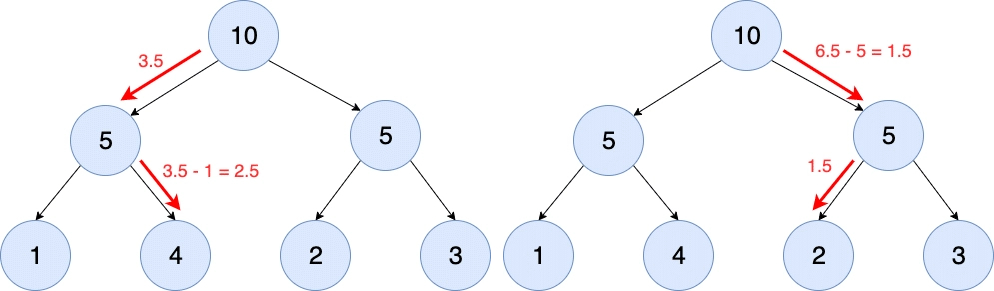
\includegraphics[scale=0.5]{img/I/Simple-SumTree-left-traverse.png}
\centering
\caption{Sum tree.}
\end{SCfigure}

\textbf{Priority update and distribution probability in the sum tree} \\
In DQN, the transitions are not consumed online, and the magnitude of the TD error $|\delta_t|$ for the current transition is unknown during exploration, it is thus stored with maximum priority $p_{max} \leq 1$ to assure that the transition is experienced at least once, i.e. the prioritized transition $(s_t,a_t,s_{t+1},r_{t+1}, p_{max})$. It is at Q-network gradient updates that the priorities $p_i^{(m)}$ are updated in the sum tree, the $M$ priorities of the prioritized transitions $(s,a,s',r',p_i)^{(m)}$ sampled in batch $P(D)$ with probability distribution $P(i)$ over the indices $i$ of the sum tree. The priorities $p_i^{(m)}$ are re-evaluated by absolute TD error, such that $p_i^{(m)}= min(|\delta^{(m)}_t| + \xi, 1)^{\eta}$, with $\xi \ll 1$, $\eta \in [0,1]$ and $p_i \in ]0,1]$. The $\eta$ coefficient determines the level of prioritization, with no prioritization for $\eta \rightarrow 0$, as all $p_i=1$, and full prioritization for $\eta \rightarrow 1$, as $p_i$ is fully dependant on the TD error magnitude. In practice, $\eta=0.6$ has been empirically found to work best. Furthermore, the sampling probability distribution over the indices $i$ in the sum tree is $P(i) = \frac{p_i}{\sum_j p_j} = \frac{p_i}{sum tree (0)}$.

\textbf{Correcting the gradient bias with importance sampling weights} \\
As the sampling probability distribution $P$ changes in an uncontrolled fashion, Per introduces a bias in learning that changes the solution that the estimates will converge to. This bias is corrected by using importance sampling (IS) weights $w_t$, to regularize the impact of over-sampled transitions on the Q-network parameters. Formally, IS weights compensate priority sampling with respect to the uniform distribution, so that prioritized transitions that are sampled as $(s,a,s',r',p) \sim P$, are experienced as $(s,a,s',r') \sim U$. The IS weights, computed over the priorities $p_i^{(m)}$ from the current batch, are $w_{t}^{(m)} = (N_t \cdot P(i))^{-\beta} / \max w_{t}$, with $Nt \leq N$ the current size of the replay memory buffer, $\beta$ a prioritization factor, and a normalization term for stability, i.e. the maximum weight for a priority in the sum tree, $\max w_{t} = (N_t \cdot \frac{p_{min}}{sum tree (0)})^{-\beta}$. As the training is highly unstable at the beginning of learning due to high randomness induced by exploration, the $\beta$ exponent controls the importance of prioritized sampling correction. In practice, $\beta$ is annealed linearly from $\beta \in [0.4,0.6]$ to $\beta=1$ over epsilon decay $\epsilon_{dec}$. The bias is then corrected by folding the IS weights $w_t$ with the TD errors $\delta_t$ in the loss function, re-adjusting the gradient $\Delta_t$ by the chain rule:
\[ L_t(\delta_t,w_t) = \frac{1}{2M}\sum_{m=1}^M w_{t}^{(m)} \cdot (\delta_t^{(m)})^2 \]

\begin{algorithm}[H]
\small
\caption*{Prioritized experience replay algorithm}
\begin{algorithmic}
    \STATE ...
    \STATE Initialize the replay memory buffer $D$ to capacity $N$
    \STATE with $Nmin$ random transitions $(s,\text{rand }a \in A,s',r')$;
    \STATE Initialize the sum tree to capacity $2N - 1$ with zero-padding;
    \FOR{step t = 1:T}
        \bindent
        \STATE ...
        \STATE Store prioritized transition $(s_t,a_t,s_{t+1},r_{t+1}, p_{max})$
        \STATE with $(s_t,a_t,s_{t+1},r_{t+1})$ in $D$ and $p_{max}$ in the sum tree;
        \STATE Sample prioritized batch $P(D)$ of $M$ transitions $(s,a,s',r',p_i)^{(m)}$, with $P(i) = \frac{p_i}{\sum_j p_j}$
        \STATE with $p_i^{(m)}$ in the sum tree and $(s,a,s',r')^{(m)}$ in $D$, with the sum tree sample algorithm;
        \FOR{m = 1:M}
            \bindent
            \STATE Set TD error $\delta^{(m)}_t = r'^{(m)} + \gamma \cdot \max_{a'}Q_{\pi,t}(s'^{(m)},a',\Theta^-_t) - Q_{\pi,t}(s^{(m)},a^{(m)},\Theta_t)$;
            \STATE Set priority $p_i^{(m)}= min(|\delta^{(m)}_t| + \xi, 1)^{\eta}$;
            \STATE Update priority $p_i^{(m)}$ in the sum tree, with the sum tree update algorithm;
            \STATE Set IS weight $w_{t}^{(m)} = (N_t \cdot P(i))^{-\beta} / \max w_{t} = (\frac{p_i^{(m)}}{p_{min}})^{-\beta}$;
            \eindent
        \ENDFOR
        \STATE Perform a gradient descent step on MSE loss $L_t(\delta_t,w_t)$ w.r.t. $\Theta_t$, with
        $\Delta_t$, $\alpha$;
        \STATE Anneal $\beta$ linearly;
        \STATE ...
    \ENDFOR
\end{algorithmic}
\end{algorithm}

\begin{algorithm}[H]
\small
\caption*{Sum tree sample algorithm, $O(\log n)$}
\begin{algorithmic}
    \STATE Initialize parent node index $i_p = 0$, left child node index $i_l = 1$, right child node index $i_r=2$;
    \STATE Initialize random uniform value $v = U(0, \sum_j p_j) = U(0, sumtree(0))$;
    \WHILE{$i_l < 2N-1$}
        \bindent
        \STATE Set $i_l = 2i_p+1$;
        \STATE Set $i_r = 2i_p+2$;
        \IF{$v > sumtree(i_l)$}
            \STATE Set $v = v - sumtree(i_l)$;
            \STATE Set $i_p = i_r$;
        \ELSE
            \STATE Set $i_p = i_l$; 
        \ENDIF
        \eindent
    \ENDWHILE
    \STATE Get transition $(s,a,s',r')$ with priority $p_i$ in $D$ at $D(i)$, with index $i=i_p - N + 1$;
\end{algorithmic}
\end{algorithm}

\begin{algorithm}[H]
\small
\caption*{Sum tree update algorithm, $O(\log n)$}
\begin{algorithmic}
    \STATE Initialize propagation index with leaf node index $i_t = i+N-1$;
    \STATE Set propagation difference value $d = p_i - sumtree(i_t)$;
    \STATE Update $p_{max} = max(p_i,p_{max})$, $p_{min} = min(p_i,p_{min})$;
    \STATE Update priority value $sumtree(i_t) = p_i$;
    \WHILE{$i_t$ not $0$}
        \bindent
        \STATE Set $i_t = \lfloor(i_t - 1) / 2\rfloor$;
        \STATE Propagate difference $sumtree(i_t) = sumtree(i_t) + d$;
        \eindent
    \ENDWHILE
\end{algorithmic}
\end{algorithm}

\textbf{Towards state of the art with rainbow DQN} \\
The rainbow DQN framework lists three additional extensions to the vanilla DQN algorithm, apart from the three discussed here. (1) Noisy DQN learns to ignore perturbations in the training data by incorporating a noisy stream to the Q-network. (2) N-step DQN accumulates a multi-step target to learn rewards over sequences of n steps, rather than immediate rewards. (3) Distributional DQN learns distributional returns instead of expected ones by minimizing the Kullback–Leibler divergence over online and target distributions. \\
When combined; i.e. vanilla DQN with double TD target, dueling NN architecture, prioritized experience replay, noisy stream, n-step reward and distributional return; the resulting algorithm is the state of the art for deep Q-learning, the rainbow DQN algorithm. 

\pagebreak